\documentclass[14,fleqn]{article}
\usepackage{amsmath}
\usepackage{amssymb}
\usepackage[top=.5 in,left=.5 in,right=.5 in,bottom=.5 in]{geometry}
\usepackage{enumerate}
\usepackage{ mathrsfs }
\usepackage{graphicx}
\usepackage{pgf,tikz}
\usepackage{mathrsfs}
\usepackage{gensymb}
\usepackage{venndiagram}
\usepackage{enumitem}
\usetikzlibrary{arrows}

\pagenumbering{gobble}

\setlength{\parindent}{0 pt}
\setlength{\parskip}{1 ex}

\newcommand{\lcm}{\textnormal{lcm}}
\newcommand{\norm}{\triangleabove right}
\newcommand{\bfm}[1]{$\boldsymbol{#1}$}
\newcommand{\Z}{\ensuremath{\mathbb{Z}}}
\newcommand{\R}{\ensuremath{\mathbb{R}}}
\newcommand{\C}{\ensuremath{\mathbb{C}}}
\renewcommand{\wedge}[1]{\ensuremath{\langle #1 \rangle}}
\newcommand{\infsum}[1]{\ensuremath{\sum_{n=#1}^\infty}}
\newcommand{\defn}[1]{\textbf{\underline{#1}}}
\newcommand{\var}{\ensuremath{\mathrm{Var}}}

%\begin{venndiagram3sets}[labelA=$S$,labelB=$T$,labelC=$U$]
%	\fillA
%	\fillOnlyC
%\end{venndiagram3sets}\\

%\begin{venndiagram2sets}[labelA=$S$,labelB=$T$]
%	\fillNotA
%	\fillNotB
%	\setpostvennhook{
%		\draw[] (labelAB) ++(0,-2.1) node {\raisebox{0pt}[0pt][0pt]{$(S\cap T)'$}};
%	}
%\end{venndiagram2sets}\\

\begin{document}
\section{Section 7.6: The Normal distribution}
So far we have only dealt with random variables that are discrete, that is they only have finitely many outcomes. But there is one distribution that is so important that we have to talk about it, and it isn't discrete.

Example: Consider the a random variable $X$ which is distributed binomially with $n=20$ and $p=1/2.$ Here is the histogram representing the probabilites of each outcome.\\
\begin{center}
	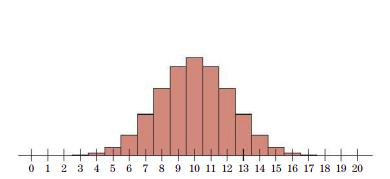
\includegraphics{binomialhistogram.jpg}
\end{center}
How would you describe this data?

A common term you might have heard is bell-shaped. In fact, we could approximate the tops of these rectangles by a bell shaped curve which is called a \defn{normal curve}. In this section we will study experiments with \defn{normally distributed outcomes}. These examples are so important because they are so common. Some examples include
\begin{itemize}
	\item Height of a random adult woman
	\item Weight of a steel beam made at a factory
	\item IQ of a random person
\end{itemize}
and many more.

What are some properties of the normal curve. The central peak occurs at at the mean $\mu$ and the curve is symmetric about this line. Suppose $X$ is a random variable with a given normal curve. There is a connection between the normal curve and the random variable $X.$ The probability that $X$ lies between $a$ and $b$ is the area under the curve between $a$ and $b.$\\
\begin{center}
	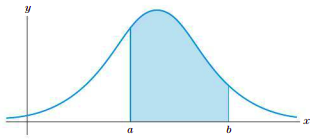
\includegraphics{normalcurve.png}
\end{center}

Notice the similarieties between this and the binomial distribution. In both cases we are computing probability via area. What is the area under a normal curve?\\
It must be 1 because we are computing a probability.

Example: Suppose $X$ is normally distributed with mean $\mu=-2.$ Draw normal curves and shade the appropriate area for the following probabilities:
\begin{enumerate}
	\item $P(X<-2)$
	\item $P(X\ge 1)$
	\item $P(-3\le X\le 0)$
	\item $P(|X|>1)$
\end{enumerate}

We know from last section that mean doesn't tell us everything. The same thing is true for a normal distribution. There are lots of normal distributions with the same mean, but what can change is how much the data is spread out. Let's look at normal distribuations with mean $\mu=0$ to begin with. Then we can have distributions that look like the following.\\
\begin{center}
	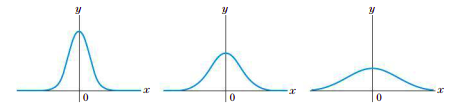
\includegraphics{differentvariance.png}
\end{center}
In this case the standard deviation $\sigma$ is what is different. It turns out, that a normal distribution has exactly two parameters, $\mu$ and $\sigma$ and they tell us everything about the distribution. This is similar to how a binomial distribution is determined by $n$ and $p.$ The value of $\sigma$ also has a geometric relationship to the graph. The normal curve changes concavity at two places, and they are exactly $\sigma$ away from the mean.

The formula for the standard normal curve is 
\[
	y=\frac{1}{\sigma\sqrt{2\pi}}e^{-\frac{(x-\mu)^2}{2\sigma^2}}
\]
which you don't need to know. Even with calculus, there is no way to find exact values for areas under this curve. So we use technology to approximate this data and compile it into tables called normal tables. However, to have one of these for each $\mu$ and $\sigma$ would take a lot of paper, so we focus on a single normal distribution.

The \defn{standard normal distribution} is the normal distribution with $\mu=0$ and $\sigma=1.$ We will denote the standard normal distribution by the random variable $Z.$ For any number $z$ we let $A(z)$ be the area under the standard normal curve to the left of $z.$ \Large put picture here \normalsize

We know that $A(z)=P(Z\le z)=P(Z<z).$ Using just the values of $A(z),$ we can actually compute any probability using 3 important facts
\begin{enumerate}
	\item The standard normal curve is symmetric about $y=0$
	\item The total area under the standard normal curve is 1.
	\item $P(Z\le z)=A(z)$
\end{enumerate}
So we make a table of values for $A(z)$ and work from there.\\
Example: Write the following probabilities in terms of $A(z).$ (You may have to add and subtract.)
\begin{enumerate}
	\item $P(Z<1)$
	\item $P(Z>-2)$
	\item $P(Z>0.5)$
	\item $P(-1<Z<2)$
	\item $P(|Z|>2)$
\end{enumerate}

Example: Suppose you have a stock that will make some ammount of money each day. The ammount of money you make each day is distributed standard normally in dollars. Find the probability that the stock will make more than \$1.75 on a given day.\\
We want $P(Z>1.75)=P(Z<-1.75)=0.0401$ which we can read off the table.

We have another definition which is relevant. If $X$ is a random variable then we say that a value $s$ is the $p^\text{th}$ percentile of $X$ if $P(X<s)=p\%$ and $P(X>s)=(1-p)\%.$ The 50th percentile is known as the median. Be careful with these as they only really make sense in a normal distirbution.

Example: Find the 5th, 25th, and 90th percentile of the standard normal distribution.\\
To do this we look for the values in the normal table which are closest to the desired value. So we get the 5th percentile is -1.75, the 25th is -0.75, and the 90th is 1.25.

Now what if our distribution is normal, but not standard normal? What can we do? Well suppose $X$ is a normal distribution with mean $\mu$ and standard deviation $\sigma.$ So $E(X)=\mu$ and $\sigma_X=\sigma.$ Then compute
\[
	E\left(\frac{X-\mu}{\sigma}\right)\text{ and }\sqrt{\var(\frac{X-\mu}{\sigma})}
\]
What do you notice? It turns out that $(X-\mu)/\sigma$ is also a normal distribution and thus it is a standard normal distribution. Thus using a little algebra we get the following fact.
\[
	P(a\le X\le b)=P\left(\frac{a-\mu}{\sigma}\le \frac{X-\mu}{\sigma}\le \frac{b-\mu}{\sigma}\right)=P\left(\frac{a-\mu}{\sigma}\le Z\le \frac{b-\mu}{\sigma}\right)
\]
and it also works if $a$ or $b$ is omitted. Thus we can compute any normal probability in terms of a standard normal probability.

Example: Suppose that scores for the first exam were normally distributed with mean 88 and standard deviation 4. Find the probability that a random score was higher was an A.\\
We want to know $P(X\ge 90)=P(Z\ge (90-88)/4)=P(Z\ge 1/2)=30.85\%.$

Example: Approximate the percent of the class that got worst than a B. What score would you need to get to ensure you did better than 40\% of the class?\\

The first part is similar to the previous example, $P(X<80)=P(Z<-2)=2.28\%.$ For the second question we need to find $a$ such that $P(X<a)=0.4.$ If we do the same thing in reverse we want $P(Z<(a-\mu)/\sigma)<0.4$ which is exactly the 40th percentile. So $(a-\mu)/\sigma=-1/4$ and thus $a=(-1/4)\cdot 4+88=87.$

This idea gives the following result: If $x_p$ is the pth percentile of a normal distribution with mean $\mu$ and standard deviation $\sigma$ then\[
	x_p=\mu+z_p\sigma
\]
where $z_p$ is the pth percentile of a standard normal distribution.

Example: Suppose bolts are manufactured in such a way that the average bolt length is 1 inch and the standard deviation is 5 thousandths of an inch. What is the probability that a randomly selected bolt is more than 2 thousandts of an inch shorter than it should be?\\
\[
	P(X<1-0.002)=P(Z<-0.4)=0.3446
\]

\end{document}
